\chapter{Efecto Kerr magneto-\'optico} \label{cap:Kerr}
\section{Introducci\'on al efecto Kerr magneto-\'optico} \label{Kerr:sec:Intr}
Una manera de estudiar las propiedades magn\'eticas de los materiales es haciendo uso de los efectos magneto-\'opticos, los cuales surgen como resultado de la interacci\'on entre la luz y la materia que es sujeta a un campo magn\'etico y que en el caso de materiales que tengan cierto orden magn\'etico, tales como los materiales ferromagn\'eticos, se siguen observando estos fen\'omenos en el caso de que no se apliquen campos magn\'eticos externos. Dichos fen\'omenos provienen de la separaci\'on de niveles de energ\'ia inducidos por la aplicaci\'on de un campo magn\'etico externo; es decir proviene del efecto Zeeman y lo cual provoca que cambie el espectro del coeficiente de  absorbci\'on y tiende a la aparici\'on o a la variaci\'on de la anisotropía magn\'etica. La anisotrop\'ia de un medio magnetizado se puede observar en la reflexi\'on de la luz en la superficie, el cual es el llamado efecto Kerr magneto-\'optico, que fue descubierto por  John Kerr en 1888 observando el cambio de polarizaci\'on  lineal a eliptica provocado por la reflexi\'on de la luz en un electroim\'an pulido \cite{Kerr_1888}.  
\newline
\par En la espectroscopia de efecto Kerr magneto-\'optico generalmente se distingue entre la polarizaci\'on lineal incidente entre $s$ y $p$, en las cuales el campo el\'ectrico est\'a normal ($s$) o paralelo ($p$) al plano de incidencia y estas propiedades magneto-\'opticas dependen de las polarizaciones $s$ y $p$ \cite{mo_2004}.
\newline
\par Se pueden caracterizar tres tipos de  efecto Kerr dependiendo de la orientaci\'on del vector de magnetizaci\'on con respecto a la superficie y al plano de incidencia del haz: polar, longitudinal y transversal, los cuales se observan en la figura \ref{Kerr:fig:Conf}. La configuraci\'on polar (fig. \ref{Kerr:fig:pol}) se tiene cuando el vector de magnetizaci\'on se orienta en la direcci\'on perpendicular a la superficie del material y paralelamente al plano de incidencia. La geometr\'ia longitudinal (fig. \ref{Kerr:fig:long}) se obtiene cuando se orienta el vector de magnetizaci\'on paralelamente a la superficie del material y al plano de incidencia y la configuraci\'on transversal se da cuando se orienta perpendicularmente al plano de incidencia y  paralelamente a la superficie.  La influencia de la magnetizaci\'on el las configuraciones polar  y longitudinal provoca la rotaci\'on del plano de polarizaci\'on y la aparici\'on de  la elipticidad de la luz reflejada. En cambio en la configuraci\'on transversal, solo se observa el cambio de la intensidad y la fase del haz incidente \cite{mo_2004}.
\begin{figure}[!hbt]
	\centering
	\subfigure[polar]{
		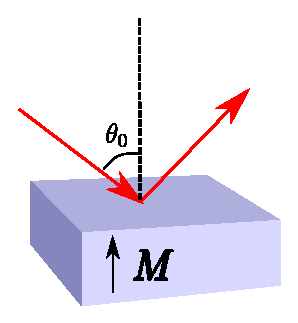
\epsfig{file=figKerr/pol/pol.eps, width=5.0cm,height=5.0cm}
		\label{Kerr:fig:pol}
	}
    \subfigure[longitudinal]{
    	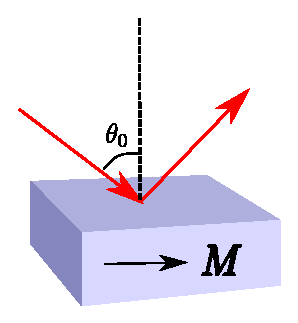
\epsfig{file=figKerr/pol/long.eps, width=5.0cm,height=5.0cm}
    	\label{Kerr:fig:long}
    }
    \subfigure[transversal]{
    	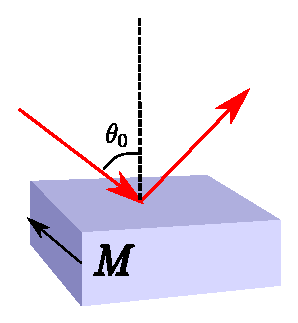
\epsfig{file=figKerr/pol/trans.eps, width=5.0cm,height=5.0cm}
    	\label{Kerr:fig:trans}
    }
   \caption[Configuraciones de Efecto Kerr magneto-\'optico.]{Diferentes configuraciones del efecto Kerr magneto-\'optico}
   \label{Kerr:fig:Conf}
\end{figure}
\newline
La constante de diel\'ectrica $\hat{\epsilon}$ se puede escribir de la siguiente forma asumiendo que las componentes $\epsilon_{xx} \approx \epsilon_{zz}$ \cite{You_1996}:
\begin{equation}
\hat{\epsilon}= \epsilon_{xx}
\begin{pmatrix}
1         & -i Q_1 m_z & i Q_2 m_y \\
i Q_1 m_z & 1          &  i Q_3 m_x\\
-i Q_2 m_y&-i Q_3 m_x  & 1
\end{pmatrix}
\label{Kerr:ec:consDiel},
\end{equation}
en donde $m_{x,y,z}$ son los cosenos directores del vector de magnetizaci\'on y
\begin{equation*}
\left(Q_1, Q_2, Q_3\right)= \left(i \frac{\epsilon_{xy}}{\epsilon_{xx}},-i \frac{\epsilon_{xz}}{\epsilon_{xx}}, -i \frac{\epsilon_{yz}}{\epsilon_{xx}} \right)
\end{equation*}
son las constantes giromagn\'eticas del material \cite{mo_2004,You_1996}. Es importante notar que las componenetes del tensor diel\'ectrico $\hat{\epsilon}_{\alpha, \beta}$ tienen componentes reales e imaginarias $\hat{\epsilon}_{\alpha, \beta} = \epsilon_{\alpha, \beta}^{(1)} +i\epsilon_{\alpha, \beta}^{(2)} $, donde $\alpha,\beta \equiv x,y,z$, $\epsilon_{xx}= (n+k)^2$,  siendo $n$ y $k$ el \'indice de refracci\'on y de extinci\'on respectivamente. El tensor diel\'ectrico se relaciona con el de la conductividad $\hat{\sigma}_{\alpha, \beta} = \sigma_{\alpha, \beta}^{(1)} +i\sigma_{\alpha, \beta}^{(2)} $ de la siguiente forma:
\begin{equation}
\hat{\epsilon}_{\alpha,\beta}(\omega)= \delta_{\alpha,\beta}+ \frac{4 \pi i}{\omega}\hat{\sigma}_{\alpha,\beta}(\omega) \label{Kerr:ec:relES}.
\end{equation}
De igual manera se puede definir el coeficiente de refracci\'on complejo $\hat{N}(\omega)$:
\begin{equation}
\hat{N} (\omega) \equiv \sqrt{\hat{\epsilon} (\omega)} = n(\omega) + k(\omega). \label{Kerr:ec:N}
\end{equation}  
Resolviendo las ecuaciones de Maxwell utilizando el tensor diel\'ectrico (ec. \ref{Kerr:ec:consDiel}) se encuentra que  la matriz de reflexi\'on de Fresnel, la cual es utilizada en el an\'alisis de Jones del ap\'endice \ref{Jones:App}, se puede escribir como:
\begin{equation}
R=
\begin{pmatrix}
\tilde{r}_{pp}  &  \tilde{r}_{ps} \\
\tilde{r}_{sp}  &  \tilde{r}_{ss}
\end{pmatrix}
\label{Kerr:ec:ref},
\end{equation}
en donde $\tilde{r}_{i,j}$ es la raz\'on entre el campo eléctrico incidente $j$ y el campo reflejado $i$, cuyas expresiones se pueden encontrar el art\'iculo de Chun-Yeol You \cite{You_1996}. Los efectos magneto-\'opticos se pueden definir en funci\'on de estos par\'ametros escribiendo el \'angulo Kerr complejo \cite{You_1996}:
\begin{subequations}
	\begin{gather}
	\Theta_K ^p = \theta_K^p + i \eta_K^p \equiv \frac{\tilde{r}_{sp}}{\tilde{r}_{pp}}, \label{Kerr:ec:AngKp} \\
	\Theta_K ^s = \theta_K^s + i \eta_K^s \equiv \frac{\tilde{r}_{ps}}{\tilde{r}_{ss}}, \label{Kerr:ec:AngKs}
	\end{gather}
\end{subequations}
en donde $\theta_K$ es el \'angulo de rotaci\'on de la polarizaci\'on  y $\eta_K$ es la elipticidad de el haz de luz, que ambas  son utilizadas para obtener las ecuaciones para el efecto Kerr en sus tres configuraciones.
\section{Efecto Kerr longitudinal} \label{Kerr:sec:long}
En el caso de la configuraci\'on longitudinal se asume que $m_x = m_z =0$ y $m_z =1$ y por lo tanto el tensor diel\'ectrico se puede escribir como:
\begin{equation}
\hat{\epsilon}= 
\begin{pmatrix}
\epsilon_{xx} & 0           &\epsilon_{xz} \\
0             &\epsilon_{xx}& 0            \\
-\epsilon_{xz}&0            &\epsilon_{xx} 
\end{pmatrix}.
\label{Kerr:ec:tensDielL}
\end{equation}
La ecuaci\'on para el \'angulo Kerr complejo con la configuraci\'on longitudinal se encuentra utilizando las ecuaciones para el caso general \cite{mo_2004}:
\begin{equation}
\Theta_K^{s,p} =-\frac{\hat{\epsilon}_{xz} \sin (\theta_0) \left(\sqrt{\hat{\epsilon}_{xx}-\sin^2(\theta_0) } \pm \sin(\theta_0) \tan(\theta_0)\right)}{(\hat{\epsilon}_{xx}-1) (\hat{\epsilon}_{xx}-\tan^2 (\theta_0))\sqrt{\hat{\epsilon}_{xx}-\sin^2(\theta_0) }}, \label{Kerr:ec:AngCompL}
\end{equation}
en donde $\theta_0$ es el \'angulo de incidencia del haz mostrado en la figura \ref{Kerr:fig:long} y los signos $(+)$  y $(-)$ corresponde a la polarizaci\'on $s$ y $p$, respectivamente. En el caso de la aproximaci\'on  $\epsilon_{xx} \approx \epsilon_{zz}$ ya no sea v\'alida se usa la siguiente expresi\'on \cite{mo_2004}:
\begin{equation}
\Theta_K^{s,p} = - \frac{2 \hat{\epsilon}_{xz} \sin (\theta_0) \cos(\theta_0) \sqrt{\hat{\epsilon}_{xx}}}{D}, \label{Kerr:ec:AngSApr}
\end{equation}
con
\begin{multline*}
D= \left(\sqrt{\hat{\epsilon}_{xx}(\hat{\epsilon}_{zz}- \sin^2(\theta_0))}+\sqrt{\hat{\epsilon}_{zz}(\hat{\epsilon}_{xx}- \sin^2(\theta_0))} \right) \times \\
\left(\sqrt{\hat{\epsilon}_{xx}- \sin^2(\theta_0)} \pm \cos(\theta_0) \right) \left(\sqrt{\hat{\epsilon}_{xx} \hat{\epsilon}_{zz}} \cos(\theta_0)\mp \sqrt{\hat{\epsilon}_{zz}- \sin^2(\theta_0)}\right).
\end{multline*}
La ecuaci\'on \ref{Kerr:ec:AngSApr} y su aproximaci\'on (ec. \ref{Kerr:ec:AngCompL}), son las expresiones fundamentales para explicar la espectroscopia del efecto Kerr magneto-\'optico.
\endinput 